\chapter{Calendar dates}
\label{chap:calendar}

\section{Introduction}
\label{sec:cal-intro}

Any software that aims to handle time-series data must have a good
built-in calendar. Gretl offers several functions to handle date and
time information, which are fully documented in the \GCR{}. In order
to use them effectively, we begin by listing the various possibilities
for storing a date either as a string or a number.

\section{Date and time representations}
\label{sec:cal-representations}

In Gretl, there are several ways to encode a piece of information such
as ``May 26th, 1993''. Some of them are more intuitive, some others
are less obvious from the viewpoint of a human, but easier to handle
for an algorithm. The basic representations we discuss here are:
\begin{enumerate}
\item the three-digits approach;
\item date as string;
\item the ISO 8601 standard;
\item the epoch day;
\item Unix-like seconds;
\end{enumerate}
First, we will briefly explain what these are; then, a description of
how to convert one into another will follow.

\subsection{The three-digit approach}
\label{sec:cal-3digits}

This is probably the most obvious way to encode a date
numerically. Assuming we are not interested in intra-day information
(the time in hours and minutes, for example), the date ``May 26th,
1993'' can be stored as
\begin{code}
  scalar y = 1993
  scalar m = 5
  scalar d = 26
\end{code}

Of course, it is perfectly possible to use gretl's multiple-element
objects to extend this approach, for example using a 3-vector for
year, month and day, or a 3 column matrix for storing as many dates as
desired. If you have to store dates as a data series in your dataset,
this approach would lead you to using three series and possibly
grouping them into a list, as in
\begin{code}
  nulldata 60
  series y = 2020
  series m = time < 32 ? 1 : 2
  series d = time - (m==2) * 31
  list DATE = y m d
\end{code}
The example above will generate daily dates for January and February
2020. In some cases, \texttt{CSV} files store dates exactly in this
format, possibly with different conventions on the ordering of the
three components.

\subsection{Date as string}
\label{sec:cal-generic-string}

To a human being, this is the most natural choice: something like
``26/6/1953'' is pretty much unambiguous. Using this format for
machine processing can be problematic for several reasons, the main
one being the existence of many different conventions on (a)
separators and (b) the order in which the three pieces of information
(day, month, year) come. Therefore, Gretl provides a fairly
comprehensive function for converting dates such as these into more
manageable formats.

\subsection{The ISO 8601 standard}
\label{sec:cal-ISO8601}

The ISO 8601 standard provides in fact two different representations
for a date: the ``basic'' representation, which uses an 8-digit
integer and the ``extended'' representation, which uses a 10-character
string.

In the basic representation, the idea is that the first four digits
represent the year, the middle two the month and the rightmost two the
day, so that for example \texttt{20170219} indicates February 2nd,
2017. The extended representation works similarly, except that the
date is a string where the items are separated by hyphens, so that the
same date would be coded as ``\texttt{2017-02-19}''.

Again, using series and/or matrices to store ISO 8601 basic dates is
trivial.

\subsection{The epoch day}
\label{sec:cal-epochday}

The third representation is as an ``epoch day'': the date is stored as
an integer, the number of days elapsed since January 1, AD 1 (that is,
the first day of the Common Era), on the proleptic Gregorian
calendar.\footnote{The term ``proleptic,'' as applied to a calendar,
  indicates that it is extrapolated backwards or forwards relative to
  its period of actual historical use.} For example, 1993-05-26
orresponds to 727709.

This is also the convention used by the \textsf{GLib} library, on
which gretl depends for most of its calendrical calculation. Since
\textsf{GLib} represents epoch days as unsigned integers, this means
that gretl does not support dates prior to the Common---or, if you
prefer, Christian---Era (see also Section \ref{sec:cal-conversion}).

This representation has sevaral advantages: like the ISO 8601 basic
representation, it lends itself quite naturally to represent dates as
data series. Compared to ISO 8601, it has the disadvantage of not
being immediately human-readable, but to compensate for that it makes
very easy to find how long a date range is.

While ISO 8601 basic dates can be used for easy comparison (which of
two dates, on a given calendar, refers to a later day?), one needs
epoch days to carry out fully fledged ``dates arithmetic.''  Epoch
days are always consecutive by construction, but 8-digit basic dates
are consecutive only within a given month; they advance by 101 minus
(days in previous month) at the start of each month other than January
and by 8870 at the start of each year.

For example, to find how many days separate 1993-05-26 from
1996-04-12, one could use
\begin{code}
  scalar dif = epochday(19960412) - epochday(19930526)
\end{code}
That said, the dedicated function \cmd{dayspan} offers a more
sophisticated tool, that can take Saturdays and Sundays into account.

\subsection{Unix-like seconds}
\label{sec:cal-seconds}

In this representation (which has been the traditional cornerstone of
date and time handling on Unix-like systems), the date is a scalar
giving the number of seconds since the start of 1970 according to
Coordinated Universal Time (UTC --- formerly known as Greenwich Mean
Time). Therefore, this format is ideal for storing fine-grained
information, including for example not only the date but the time of
day as well.

This is not human-readable (for example, the number 123456789
corresponds to Thursday, 29 Nov 1973), but again it lends itself quite
naturally to calculations. Note that this representation is hard-wired
to the UTC time zone. Therefore, it is possible that a given value
could correspond to a different dates, if evaluated in different
time zones.

\section{Converting between representations}
\label{sec:cal-conversions}

\begin{figure}[htbp]
  \centering
  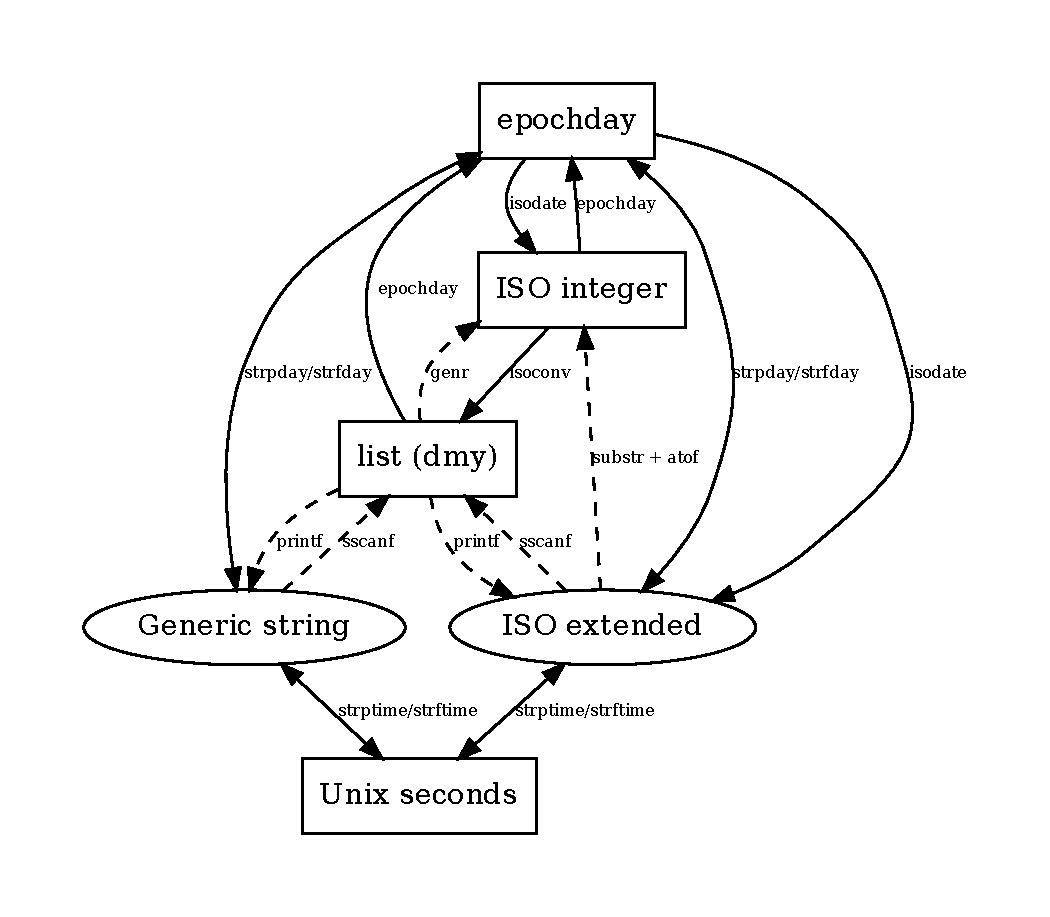
\includegraphics[scale=0.75]{figures/date-conversion}
  \caption{Conversions between different date formats}
  \label{fig:cal-conversions}
\end{figure}

In order to make the conversion between different representations,
Gretl provides several dedicated functions. In some cases, the
convwersion can be carried out by using generic functions. Figure
\ref{fig:cal-conversions} displays a summary: solid lines represent
dedicated function, while dashed lines indicate that no special
function is needed. In the rest of this section, we will discuss a few
special cases.

\subsection{Decomposing a series of ``basic'' dates}

To generate from a series of dates in ISO 8601 basic format distinct
series holding year, month and day, the function \texttt{isoconv} can
be used. This function should be passed the original series followed
by ``pointers to'' the series to be filled out. For example, if we
have a series named \texttt{dates} in the prescribed format we might
do
%
\begin{code}
series y, m, d
isoconv(dates, &y, &m, &d)
\end{code}

This is mostly just a convenience function: provided the
\texttt{dates} input is valid on the (possibly proleptic) Gregorian
calendar it is equivalent to:
%
\begin{code}
series y = floor(dates/10000)
series m = floor((dates-10000*y)/100)
series d = dates - 10000*y - 100*m
\end{code}

However, there is some ``value added'': \texttt{isoconv} checks the
validity of the \texttt{dates} input. If the implied year, month and
day for any \texttt{dates} observation do not correspond to a valid
Gregorian date in the Common Era,\footnote{For example, the implied
  month is not in the range 1--12, or the implied day is not in the
  range of 1 to the number of days in the month, taking account of
  Gregorian leap years.} then all the derived series will have value
\texttt{NA} at that observation.



\subsection{Obtaining and using epoch days}


A further---and perhaps more practical---use of epoch days is checking
whether daily data are complete. Suppose we have what purport to be
7-day daily data on the Gregorian calendar with a starting date of
2015-01-01 and an ending date of 2016-12-31. How many observations
should there be?
%
\begin{code}
ed1 = epochday(2015,1,1)
ed2 = epochday(2016,12,31)
n = ed2 - ed1 + 1
\end{code}
We find that there should be \texttt{n} = 731 observations; if there
are fewer, there's something missing. If the data are supposed to be
on a 5-day week (skipping Saturday and Sunday) or 6-day week (skipping
Sunday alone) the calculation is more complicated; in this case we can
use the \texttt{dayspan} function, providing as arguments the
epoch-day values for the first and last dates and the number of days
per week:
\begin{code}
ed1 = epochday(2015,1,1)
ed2 = epochday(2016,12,30)
n = dayspan(ed1, ed2, 5)
\end{code}
%
We discover that there were \texttt{n} = 522 weekdays in this period.

\section{Other functions and built-ins}
\label{sec:cal-otherfuncs}

\subsection{Built-ins}
\label{sec:cal-builtins}

Gretl offers you a few accessors for generating dates. One is
\dollar{now}, which returns the current date/time as a 2-element
vector: the first one is in seconds (see Section
\ref{sec:cal-seconds}) the second one is an epoch day (see Section
\ref{sec:cal-epochday}).

Moreover, when a time-series dataset is open, three accessors are
available to retrieve the dataset dates as series. \dollar{obsmajor}
normally returns the year and \dollar{obsminor} the inner subdivision
(eg the month for a monthly dataset). For daily datasets,
\dollar{obsmicro} is also available for the day. See the \GCR{} for
more details.

\subsection{Miscellaneous functions}
\label{sec:cal-misc}

Besides conversion, several other calendrical functions are available:
\begin{description}
\item[monthlen] given month and year, returns the month length in days
  (optionally ignoring weekends)
\item[weekday] given a date as year, month and day (or ISO 8601
  basic), returns a number between 0 and 7 corresponding to the weekday
  (0 is Sunday)
\item[juldate] given an epochday, returns the corresponding Julian
  date (see Section \ref{sec:cal-conversion} below) in ISO format
\item[dayspan] given two epochdays, calculate their distance,
  optionally taking weekends into account.
\item[easterday] given the year, return the date of Easter in the
  Gregorian calendar.
\item[isoweek] given a date as year, month and day, return the
  progressive number of the week within that year as per ISO 8601
  specification.
\end{description}


\section{Working with pre-Gregorian dates}
\label{sec:cal-conversion}

Working with dates is fairly straightforward in the current era, with
the Gregorian calendar now used universally for the dating of
socioeconomic observations. It is not so straightforward, however,
when dealing with historical data recorded prior to the adoption of
the Gregorian calendar in place of the Julian, an event which first
occurred in the principal Catholic countries in 1582 but which took
place at different dates in different countries over a span of several
centuries.

Gretl, like most data-oriented software, uses the Gregorian calendar
by default for all dates, thereby ensuring that dates are all
consecutive (the latter being a requirement of the ISO 8601 standard
for dates and times).\footnote{Gretl was not consistent in this regard
  prior to version 2017a: leap years were taken to be as defined by
  the Julian calendar prior to the adoption of the Gregorian calendar
  by Britain and its colonies in 1752.}

As readers probably know, the Julian calendar adds a leap day
(February 29) on each year that is divisible by 4 with no
remainder. But this over-compensates for the fact that a 365-day year
is too short to keep the calendar synchronized with the seasons. The
Gregorian calendar introduced a more complex rule which maintains
better synchronization, namely, each year divisible by 4 with no
remainder is a leap year \textit{unless} it's a centurial year (e.g.\
1900) in which case it's a leap year only if it is divisible by 400
with no remainder.  So the years 1600 and 2000 were leap years on both
calendars, but 1700, 1800, and 1900 were leap years only on the Julian
calendar. While the average length of a Julian year is 365.25 days,
the Gregorian average is 365.2425 days. 

The fact that the Julian calendar inserts leap days more frequently
means that the Julian date progressively (although very slowly) falls
behind the Gregorian date. For example, February 18 2017 (Gregorian)
is February 5 2017 on the Julian calendar. On adoption of the
Gregorian calendar it was therefore necessary to skip several days. In
England, where the transition occurred in 1752, Wednesday September 2
was directly followed by Thursday September 14.

In comparing calendars one wants to refer to a given day in terms that
are not specific to either calendar---but how to define a ``given
day''? This is accomplished by a count of days following some definite
event. Astronomers use the ``Julian Day,'' whose count starts with a
particular coincidence of astronomical cycles in the year known to the
Gregorian calendar (if one extrapolates it backwards in time) as 4714
BC.

In this section we address the problem of constructing within gretl a
calendar which agrees with the actual historical calendar prior to
the switch to Gregorian dating. Most people will have no use for
this, but researchers working with archival data may find it helpful:
it would be tricky and error-prone to enter on the Gregorian calendar
data whose dates are given on the Julian at source.

In order to represent Julian dates, Gretl uses two basic tools: one is
the \cmd{juldate} function, which conversts a Gregorian epochday into
an ISO8601-like integer and the convention that for some function,
a negative value where a year is expected acts as a ``Julian calendar
flag''.

So, for example, the following code fragment,
%
\begin{code}
edg = epochday(1700,1,1)
edj = epochday(-1700,1,1)
\end{code}
%
produces \texttt{edg} = 620548 and \texttt{edj} = 620558, indicating
that the two calendars differed by 10 days at the point in time
known as January 1, 1700, on the proleptic Gregorian calendar.

Taken together with the \texttt{isodate} and \texttt{juldate}
functions (which each take an epoch day argument and return an ISO
8601 basic date on, respectively, the Gregorian and Julian calendars),
\texttt{epochday} can be used to convert between the two calendars.
For example, what was the date in England (still on the Julian
calendar) on the day known to Italians as June 26, 1740 (Italy having
been on the Gregorian calendar since October 1582)?
%
\begin{code}
ed = epochday(1740,6,26)
english_date = juldate(ed)
printf "%.0f\n", english_date
\end{code}
%
We find that the English date was \texttt{17400615}, the 15th of June.
Working in the other direction, what Italian date corresponded to the
5th of November, 1740, in England?
%
\begin{code}
ed = epochday(-1740,11,5)
italian_date = isodate(ed)
printf "%.0f\n", italian_date
\end{code}
%
Answer: \texttt{17401116}; Guy Fawkes night in 1740 occurred on 
November 16 from the Italian point of view.

We'll now consider the trickiest case, namely a calendar which includes
the day on which the Julian to Gregorian switch occurred. If we can
handle this, it should be relatively simple to handle a purely Julian
calendar. Our illustration will be England in 1752 (a similar analysis
could be done for Spain in 1582 or Greece in 1923). A solution
is presented in Listing~\ref{ex:britain-1752}.

The first step is to find the epoch day corresponding to the Julian
date 1752-01-01 (which turns out to be 639551). Then we can create a
series of epoch days, from which we get both Julian and Gregorian
dates for 355 days starting on epoch day 639551. Note, 355 days
because this was a short year: it was a leap year, but 11 days were
skipped in September in making the transition to the Gregorian
calendar. We can then construct a series, \texttt{hcal}, which
switches calendar at the right historical point.

\begin{script}[htbp]
  \scriptcaption{Historical calendar for Britain in 1752}
  \label{ex:britain-1752}
\begin{scodebit}
# 1752 was a short year on the British calendar!
nulldata 355
# give a negative year to indicate Julian date
ed0 = epochday(-1752,1,1)
# consistent series of epoch day values
series ed = ed0 + index - 1
# Julian dates as YYYYMMDD
series jdate = juldate(ed)
# Gregorian dates as YYYYMMDD
series gdate = isodate(ed)
# Historical: cut-over in September
series hcal = ed > epochday(-1752,9,2) ? gdate : jdate
# And let's take a look
print ed jdate gdate hcal -o
\end{scodebit}
  
Partial output:
\begin{outbit}
              ed        jdate        gdate         hcal

  1       639551     17520101     17520112     17520101
  2       639552     17520102     17520113     17520102
...
245       639795     17520901     17520912     17520901
246       639796     17520902     17520913     17520902
247       639797     17520903     17520914     17520914
248       639798     17520904     17520915     17520915
...
355       639905     17521220     17521231     17521231
\end{outbit}
\end{script}

Notice that although the series \texttt{hcal} contains the correct
historical calendar (in ``basic'' form), the observation labels (in
the first column of the output) are still just index numbers. It may
be preferable to have historical dates in that role. To achieve this
we can decompose the \texttt{hcal} series into year, month and day,
then use the special \texttt{genr markers} apparatus (see
chapter~\ref{chap:datafiles}). Suitable code along with partial output
is shown in Listing~\ref{ex:britain-1752a}.

\begin{script}[htbp]
  \scriptcaption{Continuation of Britain 1752 example}
  \label{ex:britain-1752a}
Additional input:
\begin{scodebit}
series y, m, d
isoconv(hcal, &y, &m, &d)
genr markers = "%04d-%02d-%02d", y, m, d
print ed jdate gdate hcal -o
\end{scodebit}

Partial output:
\begin{outbit}
                     ed        jdate        gdate         hcal

1752-01-01       639551     17520101     17520112     17520101
1752-01-02       639552     17520102     17520113     17520102
...
1752-09-01       639795     17520901     17520912     17520901
1752-09-02       639796     17520902     17520913     17520902
1752-09-14       639797     17520903     17520914     17520914
1752-09-15       639798     17520904     17520915     17520915
...
1752-12-31       639905     17521220     17521231     17521231
\end{outbit}
\end{script}

\subsection{Year numbering}
\label{sec:cal-yearnum}

A further complication in dealing with archival data is that the year
number has not always been advanced on January 1; for example in
Britain prior to 1752, March 25 was taken as the start of the new
year. On gretl's calendar (whether Julian or Gregorian) the year
number \textit{always} advances on January 1, but it's possible to
construct observation markers following the old scheme. This is
illustrated for the year 1751 (as we would now call it) in
Listing~\ref{ex:britain-1751}.

\begin{script}[htbp]
  \scriptcaption{Historical calendar for England in 1751}
  \label{ex:britain-1751}
Input:
\begin{scodebit}
nulldata 365 # a common year
ed0 = epochday(-1751,1,1)
ed1 = epochday(-1751,3,25)
series ed = ed0 + index - 1
series jdate = juldate(ed)
series y, m, d
isoconv(jdate, &y, &m, &d)
y = ed < ed1 ? y-1 : y
genr markers = "%04d-%02d-%02d", y, m, d
print index -o
\end{scodebit}

Partial output:
\begin{outbit}
1750-01-01            1
1750-01-02            2
1750-01-03            3
...
1750-03-23           82
1750-03-24           83
1751-03-25           84
1751-03-26           85
...
1751-12-31          365
\end{outbit}

\subsection{The \cmd{weekday} and \cmd{monthlen} functions with the
  Julian calendar}

Two of the functions described in Section \ref{sec:cal-misc}, that by
default operate on the Gregorian calendar can be induced to work on
the Julian by the trick mentioned above, namely giving the negative of
the year. These are \cmd{weekday} (which takes arguments year, month
and day) and \cmd{monthlen} (which takes arguments month, year and
days per week). Thus for example
%
\begin{code}
eval weekday(-1700,2,29)
\end{code}
%
gives 4, indicating that Julian February 29, 1700 was a Thursday. And
%
\begin{code}
eval monthlen(2,-1900,5)
\end{code}
gives 21, indicating that there were 21 weekdays in Julian February
1900.


\end{script}
